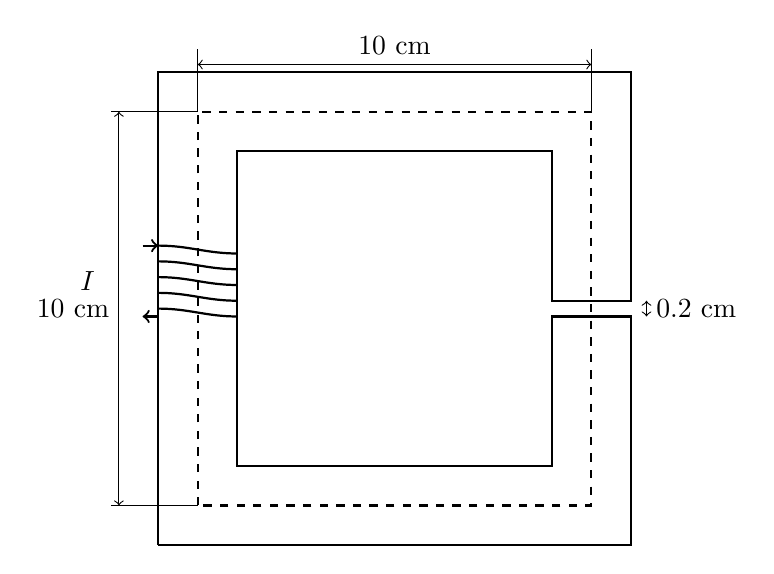
\begin{tikzpicture}
    % Define dimensions
    \def\outerwidth{5}    % Outer square width (cm)
    \def\innerwidth{9.6}   % Inner square width (10 - 0.4, considering 0.2 cm gap on each side)
    \def\gap{0.2}          % Gap size (cm)
    \def\coilspacing{0.2}  % Coil spacing (cm)
    \def\coilloops{5}      % Number of coil loops

    % Outer square
    \draw[thick] (0,0) -- (6,0) -- (6,2.9) -- (5,2.9) -- (5,1) -- (1,1) -- (1, 5) -- (5, 5) -- (5,3.1) -- (6,3.1) -- (6, 6) -- (0, 6) -- (0,0);
    %\draw[thick] 
    \draw (0.5, 5.5) -- (0.5, 6.3);
    \draw (5.5, 5.5) -- (5.5, 6.3);
    \draw (.5, .5) -- (-.6, 0.5);
    \draw (.5, 5.5) -- (-.6, 5.5);
    % Inner square
    \draw[thick, dashed] (0.5, 0.5) rectangle (5.5,5.5);

    % Winding with current I
    \foreach \i in {1,...,\coilloops} {
        \draw[thick] (1, 4 - \i * \coilspacing - \coilspacing/2) to[out=180, in=0] 
            (0, 4 - \i * \coilspacing) ;
    }

    % Label the current I
    \node at (-.9, 3.35) {$I$};

    % Dimensions
    \draw[thick][->] (-0.2, 3.8) -- (0, 3.8);
    \draw[thick][<-] (-0.2, 2.9) -- (0, 2.9);
    \draw[<->] (0.5, 6.1) -- (5.5, 6.1) node[midway, above] {10 cm};
    \draw[<->] (-.5, 0.5) -- (-.5, 5.5) node[midway, left] {10 cm};
    \draw[<->] (6.2, 2.9) -- (6.2, 3.1) node[midway, right] {0.2 cm};
\end{tikzpicture}

